\documentclass[10pt,xcolor=pdflatex,hyperref={unicode}]{beamer}
\usepackage{newcent}
\usepackage[utf8]{inputenc}
\usepackage[czech]{babel}
\usepackage[boxed,linesnumbered,noline]{algorithm2e}
\usepackage{algorithmic}
\usepackage{hyperref}

\usetheme{Madrid}
\usecolortheme{default}

\setbeamertemplate{navigation symbols}{}
\title {Pole}





\author {Igor Hanus}



\institute[FIT]
{
  {\large Fakulta informatiky\\
  VUT Brno}
}

\date {\today}

\begin{document}

\frame{\titlepage}

\begin{frame}{Čo je pole ?}
    \begin{itemize}
        \item Je to jedna z najdôležitejších datových štruktúr každého programovacieho jazyka.
        \item Hrá dôležitú rolu v ukládaní a zoraďovaní dát
        \item Jednotlivé prvky sú označované tzv. indexami.
        \item Jedinou výnimkou je jazyk Python, ktorý dokáže v poli uchovávať hodnoty rôznych typov.
    \end{itemize}
\end{frame}

\begin{frame}{Práca s poľom}
    \begin{itemize}
        \item Pod poľom si môžme predstaviť ako priehradky a každá z priehradok uchováva jeden prvok.
        \item Pre prístup k jednotlivým prvkom sa dostaneme použitím ich prideleným indexom.
        \item Idexy sú číslované od 0.
    \end{itemize}
    
    \begin{figure}
        \centering
        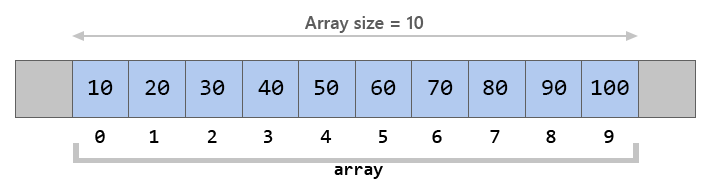
\includegraphics[scale=0.4]{array.png}
        \caption{Pole s dĺžkou 10}
    \end{figure}
\end{frame}

\IncMargin{1.5 em}
            


\begin{frame}{Inicializácia poľa}
    
    \begin{itemize}
    \item Poľu pri inicializácii môžeme napriamo pridelit hodnoty na jednotlyvé indexy.
    \end{itemize}

    \begin{algorithm}[H]
        pole$[$10$]$ $= \{10, 20, 30, 40, 50, 60, 70, 80, 90, 100\}$;
    \end{algorithm}
    \bigskip
    
    \begin{itemize}
        \item Ďalšou možnosťou je inicializácia poľa bez iniciálnzych hodnôt.
        \item Následne môžme prvky pridávať pomocou cyklu.
    \end{itemize}
    
     \begin{algorithm}[H]
        pole$[$10$]$\\
        \For{$ i = 1 $ to $ 9$} {
            \Indpp
           pole$[$ i $]$ $=$ $($ i $ + 1) * 10$;
        }
    \end{algorithm}
    
\end{frame}

\begin{frame}{Užitočné operácie s poľom}

    \begin{itemize}
    \item Hľadanie hodnoty v poli.
    \item Hľadanie najväčšej hodnoty v poli.
    \item Dvojrozmerné polia.
    \item Paralelné polia.
    \end{itemize}

\end{frame}


\begin{frame}{Hľadanie hodnoty v poli}
     \begin{algorithm}[H]
        hladane\_cislo $=$ 10\\
        pole$[$10$]$ $= \{1,8,2,9,33,7,4,9,3,1\}$\\
        \For{$ i = 1 \text{ to } 9 $} {
            \Indpp
            \uIf{$pole[\, i \,] == hladane\_cislo$}{
                return i;
            }\Else {
                return -1;
            }
            
        }
    \caption{Vrátenie indexu hľadaného čísla.}
    \end{algorithm}

\end{frame}

\begin{frame}{Hľadanie najväčšej hodnoty}
     \begin{algorithm}[H]
        
        pole$[$10$]$ $= \{1,8,2,9,33,7,4,9,3,1\}$\\
        max\_hodnota $=$ pole[0]\\
        \For{$ i = 1 \text{ to } 9 $} {
            \Indpp
            \If{$pole[\, i \,] > max\_hodnota$}{
                max\_hodnota $=$ pole$[$ i $]$;
            }
        }
        return max\_hodnota;
    \caption{Vrátenie najväčšieho prvku v poli.}
    \end{algorithm}

\end{frame}

\begin{frame}{Dvojrozmerné polia}
    \begin{itemize}
        \item Ďalšou užitočnou vlastnosťou polí je možnosť vytvorenia vnorený polí.
        \item Možnosť pracovať s maticami.
    \end{itemize}
    
    \begin{algorithm}[H]
        
        pole$[$2$]$$[$3$]$\\
    \caption{Vytvorenie matice o rozmeroch 2x3.}
    
    \end{algorithm}
    \bigskip
    
    \begin{itemize}
        \item Každý prvok ma teraz pridelené \texttt{x} a \texttt{y} súradnice, ktoré su jeho indexmi.
    \end{itemize}
    
     \begin{algorithm}[H]
        
        pole$[$0$]$$[$1$]$ $= 10$\\
        \caption{na súradnice x=1 a y=2 bol priradený prvok 10.}
    
    \end{algorithm}
    
\end{frame}

\begin{frame}{Paralelné polia}
     \begin{itemize}
         \item Vytvorenie dvoch polí, ktoré majú spoločné vlastnosti
         \item Týmto spôsobom je možné vytvoriť vzťahy medzi poľami.
         \item Jednotlivé spoločné vlastnosti majú rovnaké indexy.
     \end{itemize}

    \begin{figure}
        \centering
        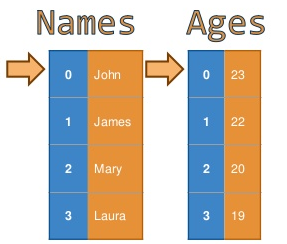
\includegraphics[scale=0.8]{parallel.png}
        \caption{Dve polia opisujúce meno a vek 4 ľudí}
    \end{figure}

\end{frame}

\begin{frame}{Zdroje}
\small
\url{https://www.itnetwork.cz/cecko/zaklady/tutorial-jazyk-c-pole}
\medskip

\url{https://medium.com/@audira98/what-is-array-2393965d047f}
\medskip

\url{https://www.cs.utah.edu/~germain/PPS/Topics/arrays.html}
\medskip

\url{https://slidetodoc.com/introduction-to-arrays-useful-array-operations-o-finding/}

\end{frame}

\end{document}